% This is the main report file

\documentclass{acm_proc_article-sp}
\usepackage[utf8]{inputenc}

\begin{document}

\title{02333 Parallel and Real-time Systems F10}
\subtitle{[Report on the work done in this course]
\titlenote{This report should also be available online at \texttt{www.notyetdecided.tld/report}}}

\numberofauthors{4} %  in this sample file, there are a *total*
\author{
% 1st. author
\alignauthor
Andreas Rask Jensen\\
%       \affaddr{}\\
%       \affaddr{}\\
       \email{s083165@student.dtu.dk}
% 2nd. author
\alignauthor
Demmus Hentze Højgaard\\
       \email{s062591@student.dtu.dk}
% 3rd. author
\alignauthor
Hjallgrim Gunnar Mohr Hentze\\
       \email{s062418@student.dtu.dk}
\and  % use '\and' if you need 'another row' of author names
% 4th. author
\alignauthor 
Kim Rostgaard Christensen\\
       \email{s084283@student.dtu.dk}
}

\maketitle
\begin{abstract}
%Abstract; A brief summary of all of the report including the conclusion section
%but excluding the acknowledgements, references and any appendixes.
The purpose of this report is to describe in detail how we implemented the tasks in the course. The overall goal is to build a tiny operating system using the technologies also available in contemporary, widely used operating systems.
\end{abstract}
% XXX Should this be here? 

% A category with the (minimum) three required fields
%\category{H.4}{Information Systems Applications}{Miscellaneous}
%A category including the fourth, optional field follows...
%\category{D.2.8}{Software Engineering}{Metrics}[complexity measures, performance measures]

%\terms{Report}

%\keywords{ACM proceedings, \LaTeX, text tagging} % NOT required for Proceedings



\section{Introduction}

%Introduction; A discussion putting the work into context and discussing the
%background of the work. The section should include any problem statements
%addressed, a very brief summary of the work carried out, the most import ant
%results and the most important conclusions. The section should end with a
%description of the report structure.


\section{Related work}
%Related work; A discussion of any material not background but still related to
%the report.

\section{Body}
This section holds the main part of the report.
%Body; A number of sections describing the work done.

Task B1 is to implement a system call. This is a pretty fundamental feature in operating systems.\\

When designing an operating system you will soon run into thoughts about security. How would you secure that only system related activities
can access the system's resources directly? Easy, some might say. Just divide it into two areas with different privilege level. 
In operating systems those two levels are called user- and kernel mode. Not all operating systems have this split, but if you have a
 lot of 3rd party development you ought to make this split.\\
Programs running in kernel mode have direct access to all I/O devices, memory and so forth. This gives a lot of possibilities (-to mess something up).\\
Programs running in user mode do not have the same privileges and need therefore to have some kind of service specified in order to communicate with I/O and get extra memory. This ``API'' is called system calls. System calls are a set of commands that the operating system listens for and when these are called the system supplies the caller with the service applied for.\\
When a syscall is invoked, the CPU registers is pushed on the stack and the OS switches to kernel mode. The kernel uses a macro that calls some low-level assembler code in order to achieve this.


\begin{figure}
\centering
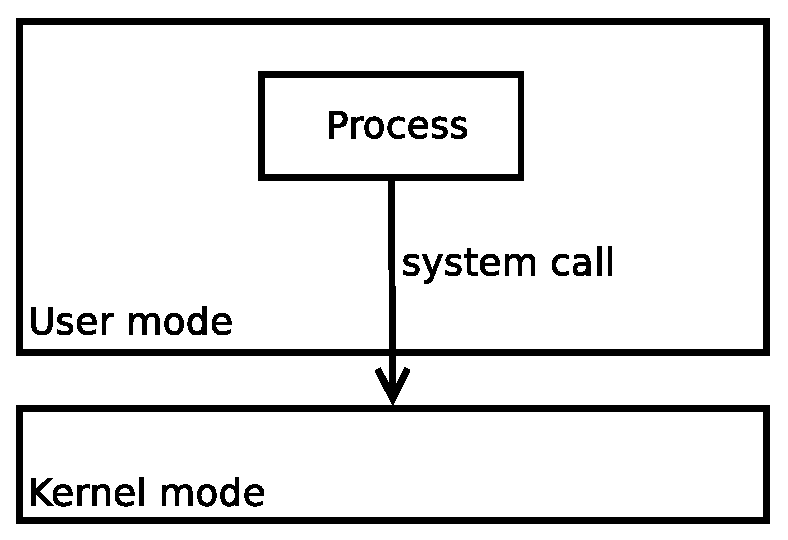
\epsfig{file=fig/Kernel_Mode.eps, height=1in}
\caption{Invoking a system call}
\label{fig:kernel_mode}
\end{figure}

\subsection{Reflections}

\subsubsection*{What kind of operating system is it?}
Tanenbaum and Woodhull describes three major types of operating system kernel types; monolithic, mico and exo.\\
The microkernel is based on the design philosophy that everything is implemented as a service, meaning that things like process management is done
in userspace and these services communicate via an IPC scheme (see section \ref{sec:ipc}).\\
%The exokernel is type of kernel that serves as a kernel on top other kernels in a hypervisor way\\
The monolithic kernel is proportionally weak in design pattern as microkernels is strong. They pretty much go by the ``anything goes'' design 
strategy. Our system is a monolithic operating system. Nothing is implemented as a service as in a microkernel or takes on any of the
characteristics of an exokernel.

%Draw a figure of the organization of the system. Relate the organization of the system to the different types of operation systems discussed in the text book by Tanenbaum and Woodhull. What kind of operating system is it?  Why?

\subsubsection*{Which portion execute in kernel mode? Which portions in user mode? What is the difference between user and kernel mode?}
All system calls is run in kernel mode. The kernel mode has access to system resources user mode doesn't

\subsubsection*{How is the kernel invoked from the user-level program? Explain and elaborate!}
The kernel is invoked through system calls. When a syscall is invoked, the CPU registers is pushed on the stack and switches to kernel mode. The kernel uses a macro that calls some low-level assembler code.

\subsubsection*{How is control passed back to the user-level program? Explain and elaborate!}

When the syscall returns, the stack is pushed back into the registers and the computer returns to user mode and continues the execution of the
program that did the system call.

\subsection{Test}
The executing program is to make the system call\\ “SYSCALL\_VERSION” where the kernel version should be printed to the bochs console. This desired result was achieved as defined in task definition, and the test was a success.

\subsection{Task B2 - processes}
Task B2 was to implement process handling in out operating system. Lets look a bit closer on the concept of processes before discussing the implementation.
\subsubsection{The process concept}
A process is a in an instance of a program (an executable) that runs in an operating system environment, 
and returns to this operating system upon completion. Hence, the operating system is the one resposible for 
creating new processes and terminating them. An analogy to this is the a java object, being an instance of a java class.\\
The process is therefore nothing more than a container for resources reserved to the process by the operating system. \\

\subsubsection{The thread concept}
A thread is the part of the process container responsible for executing the program.

So, the operating system need to keep track of the running processes and take care of creating and terminating the processes. 
For this, we have added two system calls; create and terminate.

\begin{figure}
\centering
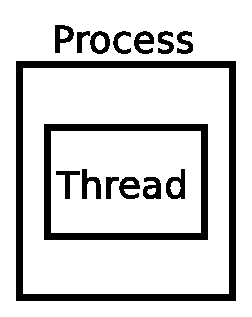
\epsfig{file=fig/Thread_Model_single.eps, width=0.5in}
\caption{Our thread model}
\end{figure}

\subsubsection*{The create system call}
To implement this, we need to keep track of the running processes. This is handled by a process table that contains structures holding information about an individual process. \\
Processes are executed invoking this system call by executing a piece of assembler code that calls a named procedure called ``main'' and then calls terminate when main is done executing.
\subsubsection*{The terminate system call}


\subsubsection{Reflections}

\subsubsection*{How is the system booted?}
Our virtual pc starts a BIOS that searches for a bootloader (in our case Grub), that then loads the kernel image to memory from a harddisk - or in our case a disk image. The kernel image 
\subsubsection*{How are processes created from executable files?}
The kernel finds all executable files and loads them to memory, storing a pointer to the first instruction for each process.

\subsubsection*{How does a daemon (process) differ from processes studied in this task?}
Our processes runs ``interactively'' and daemons runs in the background. Otherwise they share the fact that they are started at bootup by the os.


\subsection{Task B3 - scheduling}
%concepts
Task B3 was to implement a non-premptive scheduler. We will first look into at what a scheduler is and what it does.

\subsubsection{The scheduler}
A conservative definition of a CPU says that it executes code in a linear form, meaning that all program code needs to be written/executed sequentially. Therefore there can only be executed one program at once, using up all of the CPU's processing power, which often is in abundance. Today most computers have the ability to run many programs simultaneously without significant loss of performance or user experience.\\
\\
This is made possible by the scheduler, whose job is to divide the processing power of the CPU to the many processes and threads that may require it. The "simple" CPU still only manages to run its assigned code sequentially, but the scheduler can assign what code to run - That's its job.
\\
\\
\\
% Agreed - but we should write this in a comment
% !!!!!!Maybe write a short intro to scheduling algorithms!!!!!!!!
\subsubsection{Non-preemptive}
Threads are allowed to run until it is finished or goes into blocked state on its own. A thread may for example block when requesting an I/O operation or calling the sleep system call.
\\
This means that any other thread will have to wait indefinitely until all preceding threads have gone into blocked state or have finished. 

\subsubsection{Preemptive}
Instead of allowing threads to run indefinitely, we halt them during execution to allow another thread to run. For this to be viable, a hardware interrupt is required. When the scheduler interrupt is received by the CPU, it is handled by the scheduler interrupt code. The scheduler then saves all the relevant registers, including the program counter. This is referred to as a context switch, and allows return the thread and its state, at any time.

\subsubsection{Round robin}
Now that the scheduling concept is defined, we need to figure out which thread to run and when. There are many scheduling algorithms defined, all with different strengths and weaknesses. Our implementation is referred to as round robin and is a very simple in that is only cycles thru all threads in the ready state and assigns them CPU runtime. The round robin algorithm has no prioritizing in its basic implementation, and therefore all threads are treated equally in the queue and no thread is skipped or delayed CPU time.

\subsubsection{Priority}
For some "critical" applications it is more important that it gets more CPU time. These critical applications often need this extra attention, so that the user experience isn't negatively affected. An example of this is the mouse cursor, which needs to move seamlessly across the screen in a single flowing motion. Therefore many algorithms support thread prioritizing in some form, allowing highest priority threads ahead of all others with lower priority.

\subsubsection{Process states}
In this section we will explain a little about the different states that processes can have when being handled by the scheduler. Since our implementation of the kernel is able to handle multiple threads per process, we will be referring to thread states, as appose to single-threaded-processes. This just means that we do not look at processes, but just the states of individual threads. We will also in this section make the assumption, that a scheduler implements some kind of time-sharing for the CPU, so that each thread gets the same amount of processing time
\\
\\
When running multiple threads with the help of a scheduler, the CPU processing time is reduced, each time a thread is added to the scheduler queue. Since CPU time is precious, it is good practice to not waste resources on threads that don't require processing. Probably the simplest example is when code that needs to sleep/pause/wait before continuing its code execution. The program can in this case voluntary make a call to the operating system telling it to skip all its execution for a designated time period. This is also referred to as setting the thread state to blocked.
\\
\\
Another reason for halting execution is when some kind of data is missing, which is vital for continue execution. This could be that an application is waiting for I/O data, and a time delay is on that operation. Instead of having the application check for incoming data at timed intervals, we could have the operating system handle the I/O call, and block the thread until the data is available.
\\
\\
Threads can be in one of three states; running state, ready state or blocked state.
When a thread is in the running state, it is being executed by the CPU. It can from this state go to block or ready, depending on the circumstances. The ready state is for threads that are waiting for CPU time. It is then up to the scheduler which threads with ready state are executed by putting them in running state. Threads that already are in the blocked state and are designated to be run are returned to the ready state, and the scheduler takes over, as with all other threads in ready state.
\\
\\
\begin{figure}
\centering
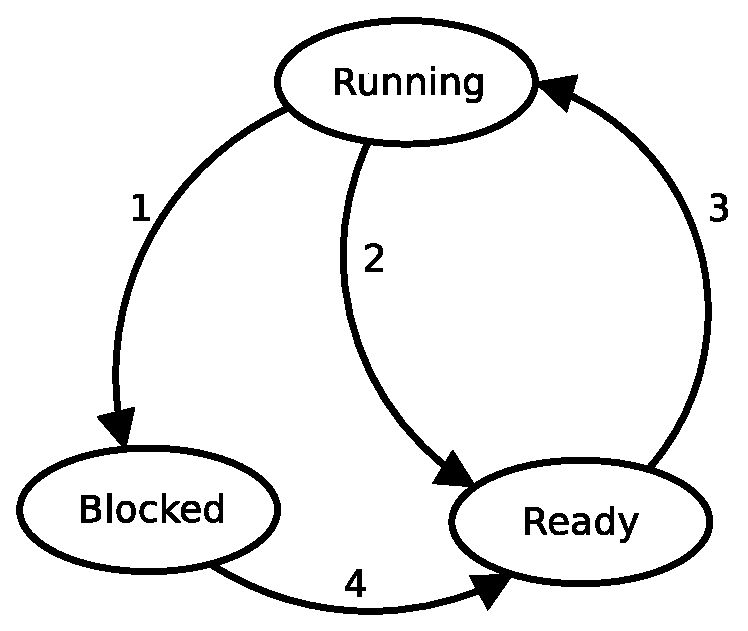
\epsfig{file=fig/Process_states.eps, height=1.5in}
\caption{Process states}
\label{fig:process_states}
\end{figure}

\subsubsection{Implementation}
\subsubsection*{scheduler.c}
The non-preemptive scheduler is implemented in the scheduler.c file, which is then included in the kernel.c file, in the system\_{}call\_{}handler() function. This means that scheduling occurs after each system call. We can also force a reschedule, which means that the currently running thread will not execute and will not be put into the ready\_{}queue. In other words the currently running thread will go into blocked state.
We make use of the variable schedule to indicate whether we want to force a rescheduling or not. If it's set to one, we don't add the currently running thread to the ready queue, i.e. the thread is in blocked state. Otherwise we enqueue the thread in the ready queue.




\subsubsection{Reflections}

\subsubsection*{What is a scheduler? What does it do and how does it work?}
A scheduler is a piece of software that shares cpu time to threads in some way. It works by keeping track of the currently running and all ready threads. If the current threads timeslot is up or it blocks, it schedules a new thread.
\subsubsection*{Assume a thread can be in three different states: running, blocked, ready. Between the states, there are various transitions. Relate the states and transitions to the code and actions in the system.}
Transition 1: The thread goes into blocked state. This is handled by the system call pause. When we call pause the thread will be inserted into the timer queue, which is a linked list of the currently paused threads, based on how many ticks it is paused for.  The head of the timer queue is the thread that has the least amount of ticks left.\\
Transition 2: The thread goes from running state to ready state. This is handled by the scheduler. The thread is enqueued into the ready queue.\\
Transition 3: The thread goes into running state. This is again handled by the scheduler. The head of the ready queue is dequeued and set to execute.\\
Transition 4: The thread goes from blocked to ready state. This is handled in the interrupt handler. It checks if there are any threads that should be woken up. If there are, it removes them from the timer queue and inserts them into the ready queue.

\subsubsection*{How does the thread queue data type work?}
The thread queue data type has a head and tail. These correspond to a thread index. It uses the next field in the thread union to construct a linked list. This linked list can then be manipulated with the functions defined in threadqueue.h.\\
\subsubsection*{How does the timer queue work?}
The timer queue is a linked list that contains all the currently paused threads. The head of the list has a list\_{}data field that specifies how many ticks are left before it should be made ready. The next thread has a list\_{}data field that contains the amount of ticks left after the previous thread has been made ready. So if we want to find out how many ticks are left before a random thread is made ready, we have to add the list\_{}data fields of all the previous thread together.\\

\section{Conclusions}
%Conclusions; All experiences and conclusions drawn from the work.
The group widely known as group 42 would like to thank everyone for their support and free coffee.\\

\subsection{Threading}
The threading works rather well, but is very limited as it only has one thread in a process. If this was to be implemented, most of the
process handling code should be rewritten.

\subsection{Scheduling}
% ready for multithreading in processes.


%ACKNOWLEDGMENTS are optional
\section{Acknowledgments}
\input{acknowledgements.tex}
%Acknowledgments; Acknowledge any persons important to the work.

%References; A list of reference material used. All material must be cited in the
%text.



% The following two commands are all you need in the
% initial runs of your .tex file to
% produce the bibliography for the citations in your paper.
\bibliographystyle{abbrv}
\bibliography{sigproc}  % sigproc.bib is the name of the Bibliography in this case
% You must have a proper ".bib" file
%  and remember to run:
% latex bibtex latex latex
% to resolve all references
%
% ACM needs 'a single self-contained file'!
%
%APPENDICES are optional
%\balancecolumns
\appendix
%Appendix A

%Appendixes; Appendixes holds, for example, results or figures that are not
%relevant to place in the body of the report. Appendixes should generally be
%avoided and might not be read by the course staff.


\section{Code examples}

\end{document}
